\section{Lecture 8: An example of reconstructor }

\subsection{Introduction}
In the previous lecture, we discussed about a practical recontructor and its various properties. In this lecture, we discuss about a simple RC circuit which behaves as a reconstructor. We also discuss the magnitude response of an RC circuit, plot its graph and the limitations of ideal sampling.  

\subsection{An Example: RC circuit}
In this lecture, the concept of sampling and reconstruction is made practical and physically realizable. The simple RC combination is used as a reconstructor. The following figure depicts an RC circuit:


\begin{figure}[ht]
\centering
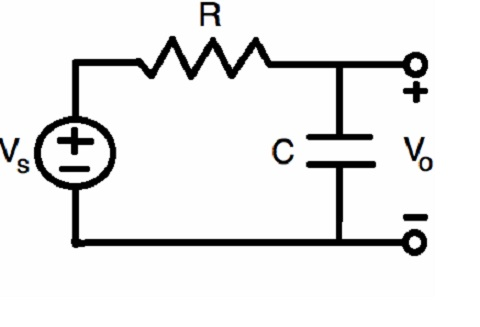
\includegraphics[width=0.3\textwidth]{circuit_RC_1.jpg}
\caption{RC circuit.}
\end{figure}

\subsubsection{Graphical approach to calculate rate of change of frequency response}

\noindent The frequency response of the given circuit is H($\Omega$).\\
Let $\Omega$ be the angular frequency.\\
Let $\tau$ = RC.\\
Then,\\ 
H($\Omega$)=$\frac{1}{1+jRC\Omega}$\\
\\
\large Magnitude of frequency response of the RC circuit is  \\

|H($\Omega$)|= $[\frac{1}{(1+(\tau \Omega)^2)}]^{1/2}$\\

\noindent Therefore the graph of the magnitude response of the RC circuit is as shown below:\\

\begin{figure}[ht]
\centering
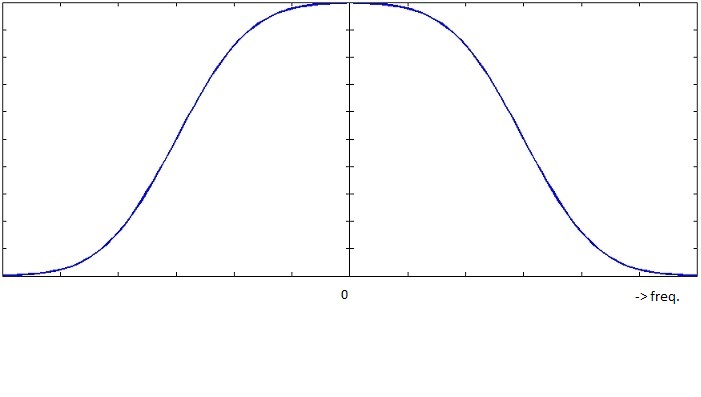
\includegraphics[width=0.3\textwidth]{graph_1_module_3.jpg}
\caption{Magnitude response of RC circuit}
\end{figure}

\noindent From the graph it is clear that the rate of magnitude change is less near 0, then increases for some time and then the rate of magnitude change again reduces and tends to 0. 

\subsubsection{Analytic approach to calculate rate of change of frequency response}

Now we try to algebraically obtain the rate of change of magnitudes at various instants.

Taking derivative of H($\Omega$),\\
$\frac{d}{d\Omega}$|H($\Omega$)|=-$\frac{1}{2}$[$1+(\Omega \tau)^2$]$^{-3/2}$. $\frac{d}{d\Omega}[1+(\tau \Omega)^2]$
\\      
\vspace*{5mm}
=
$\frac{-\tau^2\Omega}{[1+(\tau\Omega)^2]^{3/2}}$

\noindent
Case 1:\\
Now from the equation we can see that as \\ $\Omega \rightarrow$ 0,\\
$\frac{d}{d\Omega}|H(\Omega)|$ $\rightarrow$ 0.


\vspace*{0.3 cm} 
\noindent
Case 2:\\
As $\Omega \rightarrow \infty$,\\
$\frac{d}{d\Omega}H(\Omega) \approx$ $\frac{\Omega}{\Omega^3} \approx $ $\frac{1}{\Omega^2}$

\vspace*{3 mm}
\noindent
Hence, 
	$\frac{d}{d\Omega}H(\Omega) \rightarrow 0$
\\ 
\vspace*{0.5 cm}

Hence the rate of frequency response is very less near 0 and also when the values are very large, as indicated by the graph.

\subsection{Properties of a realizable reconstructor}

RC circuit is a simple and effective reconstruct.
A stable and physically realizable reconstructor must NOT have:\\
1. A completely flat region.\\
2. A region of brickwall.\\
3. Completely zero magnitude region.\\

For a perfect reconstructor the response must become 0 after a certain interval, effectively after $f_s$/2. This is not possible for a RC circuit as it does have a non zero response after $f_s$/2.
As there are no completely flat surfaces the following errors occur:\\
1. As the frequency response has no flat region, the reconstructed signal will have slight distortions.\\
2. As the reconstructor does not have zero response, the carbon copies also have an effect in the reconstructed signal.\\

To reduce these problems of ideal sampling, non-ideal sampling is used. The next session discusses about these practical non-ideal sampling.

